%yright 2007, 2008, 2009 Elsevier Ltd
%% 
%% This file is part of the 'Elsarticle Bundle'.
%% ---------------------------------------------
%% 
%% It may be distributed under the conditions of the LaTeX Project Public
%% License, either version 1.2 of this license or (at your option) any
%% later version.  The latest version of this license is in
%%    http://www.latex-project.org/lppl.txt
%% and version 1.2 or later is part of all distributions of LaTeX
%% version 1999/12/01 or later.
%% 
%% The list of all files belonging to the 'Elsarticle Bundle' is
%% given in the file `manifest.txt'.
%% 

%% Template article for Elsevier's document class `elsarticle'
%% with numbered style bibliographic references
%% SP 2008/03/01

% \documentclass[preprint,11pt]{elsarticle}
\documentclass[final,1p,11pt]{elsarticle}

%\documentclass[final,1p,times]{elsarticle}


%% Use the option review to obtain double line spacing
%%\documentclass[authoryear,preprint,review,12pt]{elsarticle}

%% Use the options 1p,twocolumn; 3p; 3p,twocolumn; 5p; or 5p,twocolumn
%% for a journal layout:
%% \documentclass[final,1p,times]{elsarticle}
%% \documentclass[final,1p,times,twocolumn]{elsarticle}
%% \documentclass[final,3p,times]{elsarticle}
%% \documentclass[final,3p,times,twocolumn]{elsarticle}
%% \documentclass[final,5p,times]{elsarticle}
%% \documentclass[final,5p,times,twocolumn]{elsarticle}

%%% For including figures, graphicx.sty has been loaded in
%% elsarticle.cls. If you prefer to use the old commands
%% please give \usepackage{epsfig}


\usepackage{epsfig}
%\usepackage{cite}
%\usepackage{mcite}
\usepackage{array,tabularx,epsfig,mathrsfs,graphicx,rotating}
\usepackage{ifthen}
\usepackage{amsfonts}
\usepackage{ragged2e}
\PassOptionsToPackage{hyphens}{url}
\usepackage[hyphens]{url}
\usepackage{hyperref}
\usepackage{listings}
\usepackage{lineno}
\usepackage{subfigure}
\usepackage{epstopdf}
% Custom colors
\usepackage{color}
\usepackage{float}
\usepackage{verbatim}

% to cross text
\usepackage[normalem]{ulem} % either use this (simple) or
\usepackage{soul} % use this (many fancier options)


\hypersetup{
  colorlinks=true,
  linkcolor=blue,
  citecolor=blue,
  urlcolor=blue
}




\graphicspath{{figs/}}


\pdfinfo{
   /Author (Chekanov et al)
   /Title  (Studies of granularity of a hadronic calorimeter for tens-of-TeV jets  at a 100 TeV pp collider)
   /CreationDate (D:2017)
   /Subject (PDFLaTeX)
   /Keywords (PDF;LaTeX)
}


\textheight=22cm
\textwidth=14.5cm

\newcommand{\beq}{\begin{equation}}
\newcommand{\eeq}{\end{equation}}
\newcommand{\la}{\langle}
\newcommand{\promc}{{\sc ProMC}}
\newcommand{\ra}{\rangle}
\newcommand{\eps}{\epsilon}
\newcommand{\ud}{\mathrm{d}}
\newcommand{\Ec}{\mathcal{E}}
\newcommand{\Fc}{\mathcal{F}}
\newcommand{\Za}{\mathrm{Z_1}}
\newcommand{\Zb}{\mathrm{Z_2}}
\newcommand{\Zn}{\mathrm{Z_n}}
\newcommand{\F}{\mathrm{F}}

\chardef\til=126
\newcommand{\GEANTfour} {\textsc{geant4}}
\newcommand{\pythia} {\textsc{Pythia8~}}
\newcommand{\pt}{\ensuremath{p_{\mathrm{T}}}}

\journal{XXX-XXX}



\begin{document}

\definecolor{mygreen}{rgb}{0,0.6,0} \definecolor{mygray}{rgb}{0.5,0.5,0.5} \definecolor{mymauve}{rgb}{0.58,0,0.82}

\lstset{ %
 backgroundcolor=\color{white},   % choose the background color; you must add \usepackage{color} or \usepackage{xcolor}
 basicstyle=\footnotesize,        % the size of the fonts that are used for the code
 breakatwhitespace=false,         % sets if automatic breaks should only happen at whitespace
 breaklines=true,                 % sets automatic line breaking
 captionpos=b,                    % sets the caption-position to bottom
 commentstyle=\color{mygreen},    % comment style
 deletekeywords={...},            % if you want to delete keywords from the given language
 escapeinside={\%*}{*)},          % if you want to add LaTeX within your code
 extendedchars=true,              % lets you use non-ASCII characters; for 8-bits encodings only, does not work with UTF-8
 keepspaces=true,                 % keeps spaces in text, useful for keeping indentation of code (possibly needs columns=flexible)
 frame=tb,
 keywordstyle=\color{blue},       % keyword style
 language=Python,                 % the language of the code
 otherkeywords={*,...},            % if you want to add more keywords to the set
 rulecolor=\color{black},         % if not set, the frame-color may be changed on line-breaks within not-black text (e.g. comments (green here))
 showspaces=false,                % show spaces everywhere adding particular underscores; it overrides 'showstringspaces'
 showstringspaces=false,          % underline spaces within strings only
 showtabs=false,                  % show tabs within strings adding particular underscores
 stepnumber=2,                    % the step between two line-numbers. If it's 1, each line will be numbered
 stringstyle=\color{mymauve},     % string literal style
 tabsize=2,                        % sets default tabsize to 2 spaces
 title=\lstname,                   % show the filename of files included with \lstinputlisting; also try caption instead of title
 numberstyle=\footnotesize,
 basicstyle=\small,
 basewidth={0.5em,0.5em}
}


\begin{frontmatter}

\title{
Studies of granularity of a hadronic calorimeter for tens-of-TeV jets  at a 100~TeV $pp$ collider 
}
%%%%%%%%%%%%%%%%%%%%%%%%%%%%%%%%%%%%%%%%%%%%%%%%%%%%%%%%%%%%%%%

\author[add3]{C.-H. Yeh}
\ead{jwzuzelski18@gmail.com}

\author[add1]{S.V.~Chekanov}
\ead{chekanov@anl.gov}

\author[addDuke,add2]{A.V.~Kotwal}
\ead{ashutosh.kotwal@duke.edu}

\author[add1]{J.~Proudfoot}
\ead{proudfoot@anl.gov}

\author[addDuke]{S.~Sen}
\ead{sourav.sen@duke.edu}

\author[add2]{N.V.~Tran}
\ead{ntran@fnal.gov}

\author[add3]{S.-S.~Yu}
\ead{syu@cern.ch}

\address[add3]{
Department of Physics, National Central University, Chung-Li, Taoyuan City 32001, Taiwan
}

\address[add1]{
HEP Division, Argonne National Laboratory,
9700 S.~Cass Avenue,
Argonne, IL 60439, USA. 
}

\address[addDuke]{
Department of Physics, Duke University, USA
}

\address[add2]{
Fermi National Accelerator Laboratory
}

\address[addMSU]{
Department of Physics, Michigan State University, 220
Trowbridge Road, East Lansing, MI 48824 
}




\begin{abstract}
Jet substructure variables for hadronic jets with transverse momenta in the range from 2.5~TeV to 20~TeV
were studied using several designs for spacial size of calorimeter cells. The studies  used 
the full Geant4 simulation 
of calorimeter response combined with realistic reconstruction of calorimeter clusters used 
in jet reconstruction. 
The results indicate that the performance of jet-substructure reconstruction 
improves with reducing cell sizes. 

\end{abstract}

\begin{keyword}
multi-TeV physics, $pp$ collider, future hadron colliders, FCC, SppC
\end{keyword}



\end{frontmatter}


% put line numbers
\linenumbers

%%%%%%%%%%%%%%%%%%%%%%%%%%%%%%%%%%%%%%%%%%%%%%%%%%%%%%%%%%%%%%%%%%
\section{Introduction}
%%%%%%%%%%%%%%%%%%%%%%%%%%%%%%%%%%%%%%%%%%%%%%%%%%%%%%%%%%%%%%%%%%

Particle collisions at energies  beyond those attained at the LHC will lead to many challenges for detector technologies.
Future experiments, such as high-energy LHC (HE-LHC),
future circular $pp$ colliders of the European initiative, FCC-hh~\cite{Benedikt:2206376} and the Chinese initiative, SppC~\cite{Tang:2015qga} will be required to measure high-momentum bosons ($W$, $Z$, $H$) and top quarks with strongly 
collimated decay products that form jets.  Studies of jet substructure can help identify such particles.

The reconstruction of jet substructure  variables for collimated jets with transverse momentum above 10 TeV 
require an appropriate detector design. The most important for reconstruction of such jets are tracking and calorimeter.
Recently, a number of studies \cite{Calkins:2013ega,Chekanov:2015ihl,Coleman:2017fiq} 
have been discussed using various fast simulation tools, such as 
Delphes  \cite{deFavereau:2013fsa}, in which momenta of particles
are smeared to mimic detector response. 

A major step towards the usage of full Geant4 simulation to verify the granularity requirements 
for calorimeters was made in \cite{Chekanov:2016ppq}.
The studies included in this paper have illustrated a significant impact 
of granularity of electromagnetic (ECAL) and hadronic (HCAL) calorimeters on the
shape of hadronic showers  calculated using calorimeter hits 
for two particles separated  by some angle. It was concluded that high granularity is essential 
in resolving two close-by particles for energies above 100 GeV. 

This paper makes another step in  understanding of this problem in terms 
of high-level physics quantities typically used in physics analyses.
Similar to the studies presented in \cite{Chekanov:2016ppq}, this paper is based on a full
Geant4 simulation with realistic jet reconstruction.

\section{Simulation of detector response and event reconstruction}
 
The description of the detector and software used for this study is discussed in \cite{Chekanov:2016ppq}. 
We use the SiFCC detector geometry with a software package that
represents a versatile environment for simulations
of detector performance, testing new technology options, event reconstruction techniques for future
100~TeV colliders.

The \GEANTfour\ (version 10.3)~\cite{Allison2016186} simulation of calorimeter response was complemented 
with the full reconstruction of calorimeter clusters formed by the Pandora algorithm \cite{Charles:2009ta,Marshall:2013bda}.
Calorimeter clusters were built from calorimeter hits in the  ECAL and HCAL after applying the corresponding sampling fractions.
No other corrections are applied.
Hadronic jets were 
reconstructed with the {\sc FastJet} package~\cite{fastjet} using the anti-$k_T$ algorithm \cite{Cacciari:2008gp}
with  a distance parameter of 0.5. 

In the following discussion, we use the simulations of a heavy $Z'$ boson, 
a hypothetical gauge boson  that arises from extensions of the electroweak symmetry of the Standard Model.
The $Z'$ bosons were simulated with the masses, $M=5$, $10$, $20$ and $40$~TeV. The lowest value 
represents a typical mass that is within the reach of the LHC experiments. The  value $40$~TeV 
represents the physics reach for a  100~TeV collider. The $Z'$ particles are forced to decay 
to two light-flavor jets ($q\bar{q}$), $W^+W^-$ or $t\bar{t}$, where
$W$ and $t$ decay hadronically. In all such scenarios, two highly boosted
jets are produced,  which are typically back-to-back in the laboratory frame.
Typical transverse momenta of such jets are $\simeq M/2$.
The main difference between considered decay types lays in different jet substructure. In the case of the $q\bar{q}$ decays,
jets do not have any internal structure. In the case of  $W^+W^-$, each jet  originates from $W$, thus it has two
subjects because of the decay $W\rightarrow q\bar{q}$. In the case of hadronic top decays, jets have three subjects due
to the decay $t \rightarrow  W^+\>b \rightarrow q\bar{q} b$.    
The signal events were generated using the \pythia generator with the default settings,
ignoring interference with SM processes.
The event samples used in this paper are  available from the
HepSim  database~\cite{Chekanov:2014fga}.



%%%%%%%%%%%%%% sections 
\section{Studies of jet properties}
\label{sec:jets}

First let us consider several variables that represent jet substructure using different types
of calorimeter granularity. The question we want to answer is how close the reconstructed
jet substructure variables to the input "truth" value that are reconstructed using 
input particles directly from the \pythia generator.


The effective radius is the average of the energy weighted radial distance in $\eta-\phi$ space of jet constituents.
Recently, it has been studied for multi-TeV jets in Ref.\cite{Auerbach:2014xua}.
 

\begin{figure}
\begin{center}
   \subfigure[5 TeV] {
   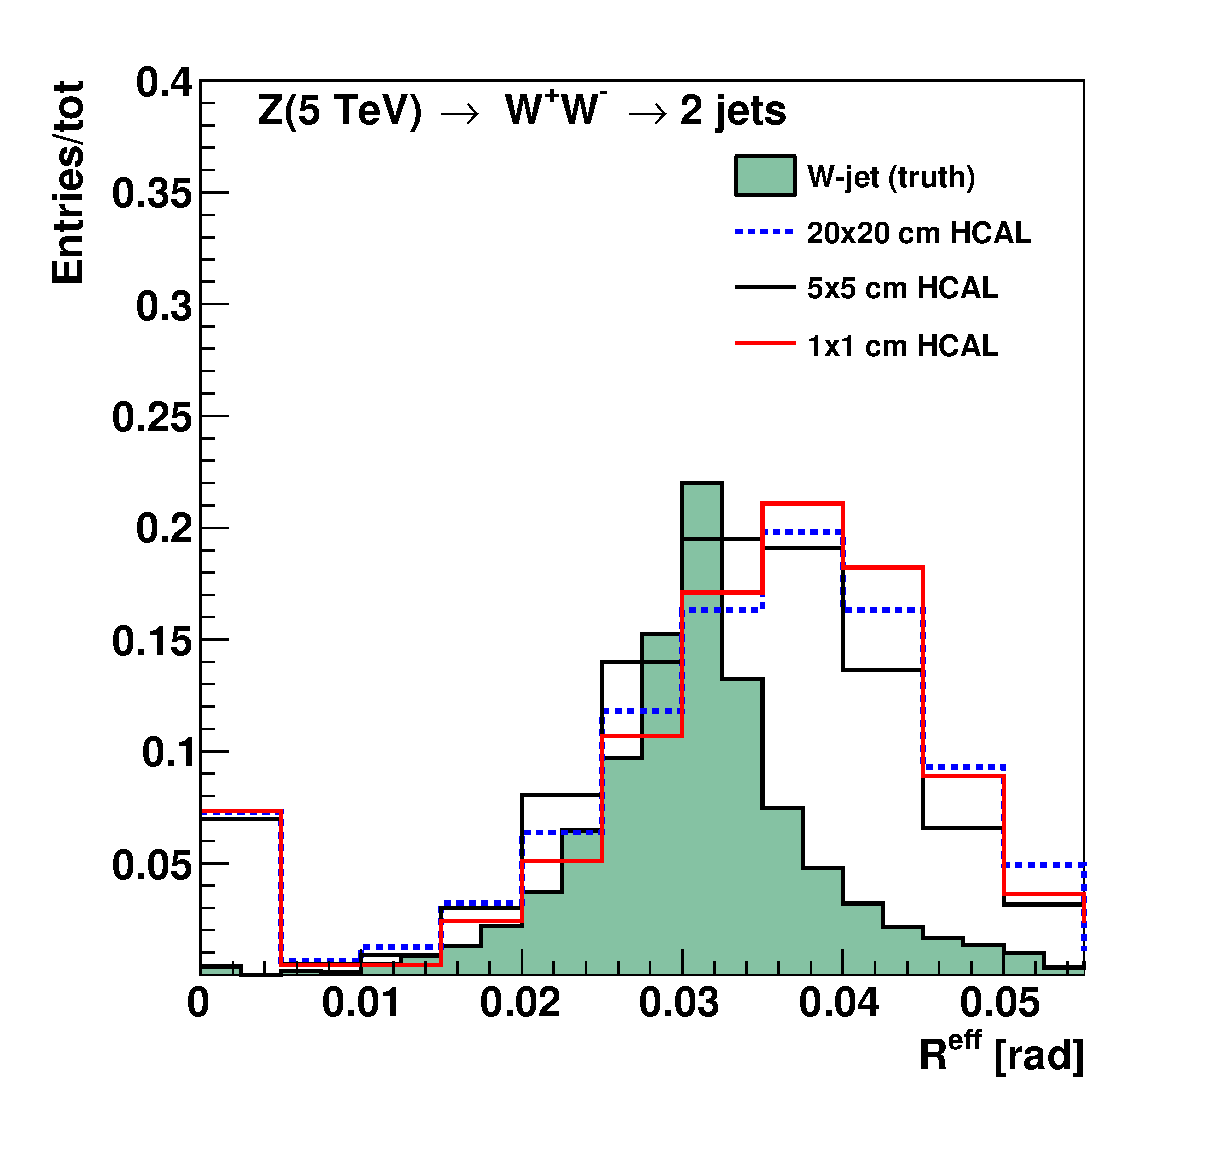
\includegraphics[width=0.43\textwidth]{figs/h5tev_clus_effR_ww1}\hfill
   }
   \subfigure[10 TeV] {
   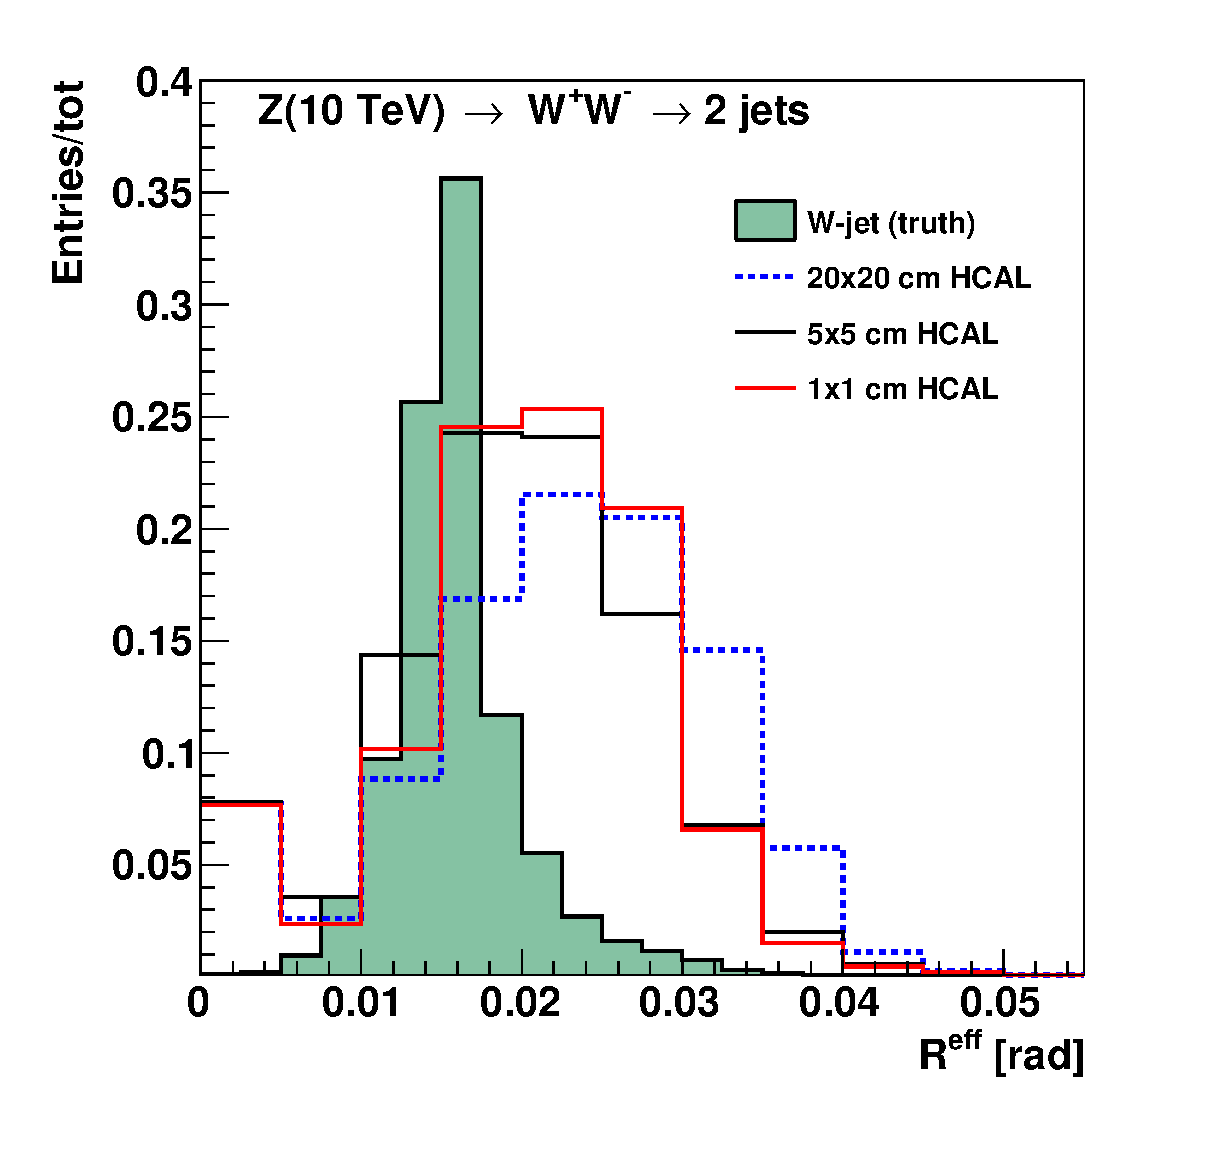
\includegraphics[width=0.43\textwidth]{figs/h10tev_clus_effR_ww1}
   }
   \subfigure[20 TeV] {
   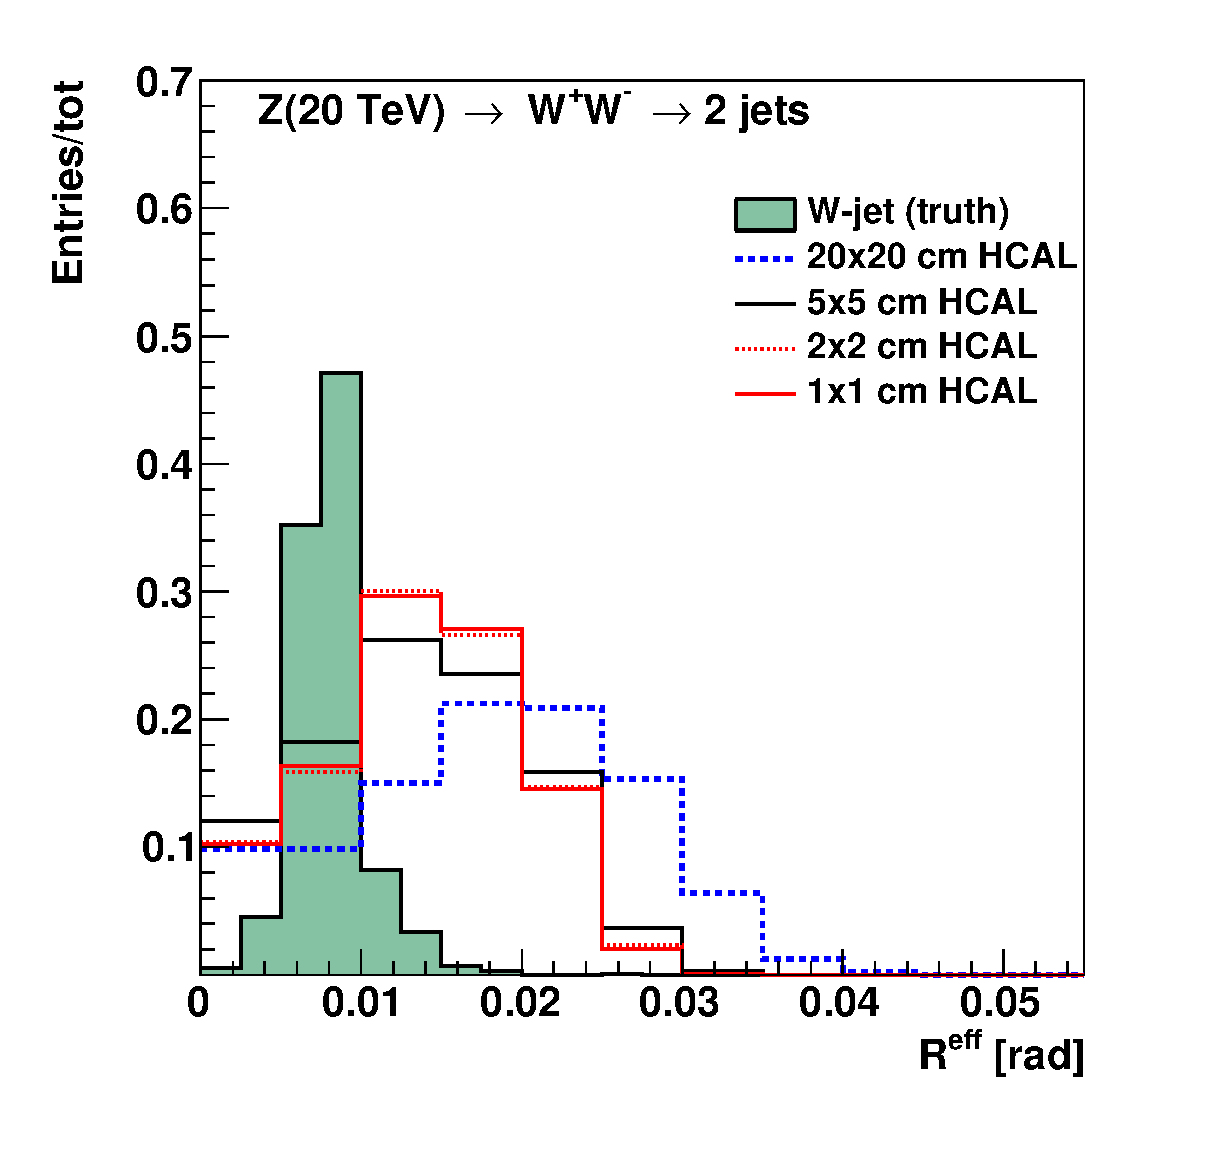
\includegraphics[width=0.43\textwidth]{figs/h20tev_clus_effR_ww1}
   }
   \subfigure[40 TeV] {
   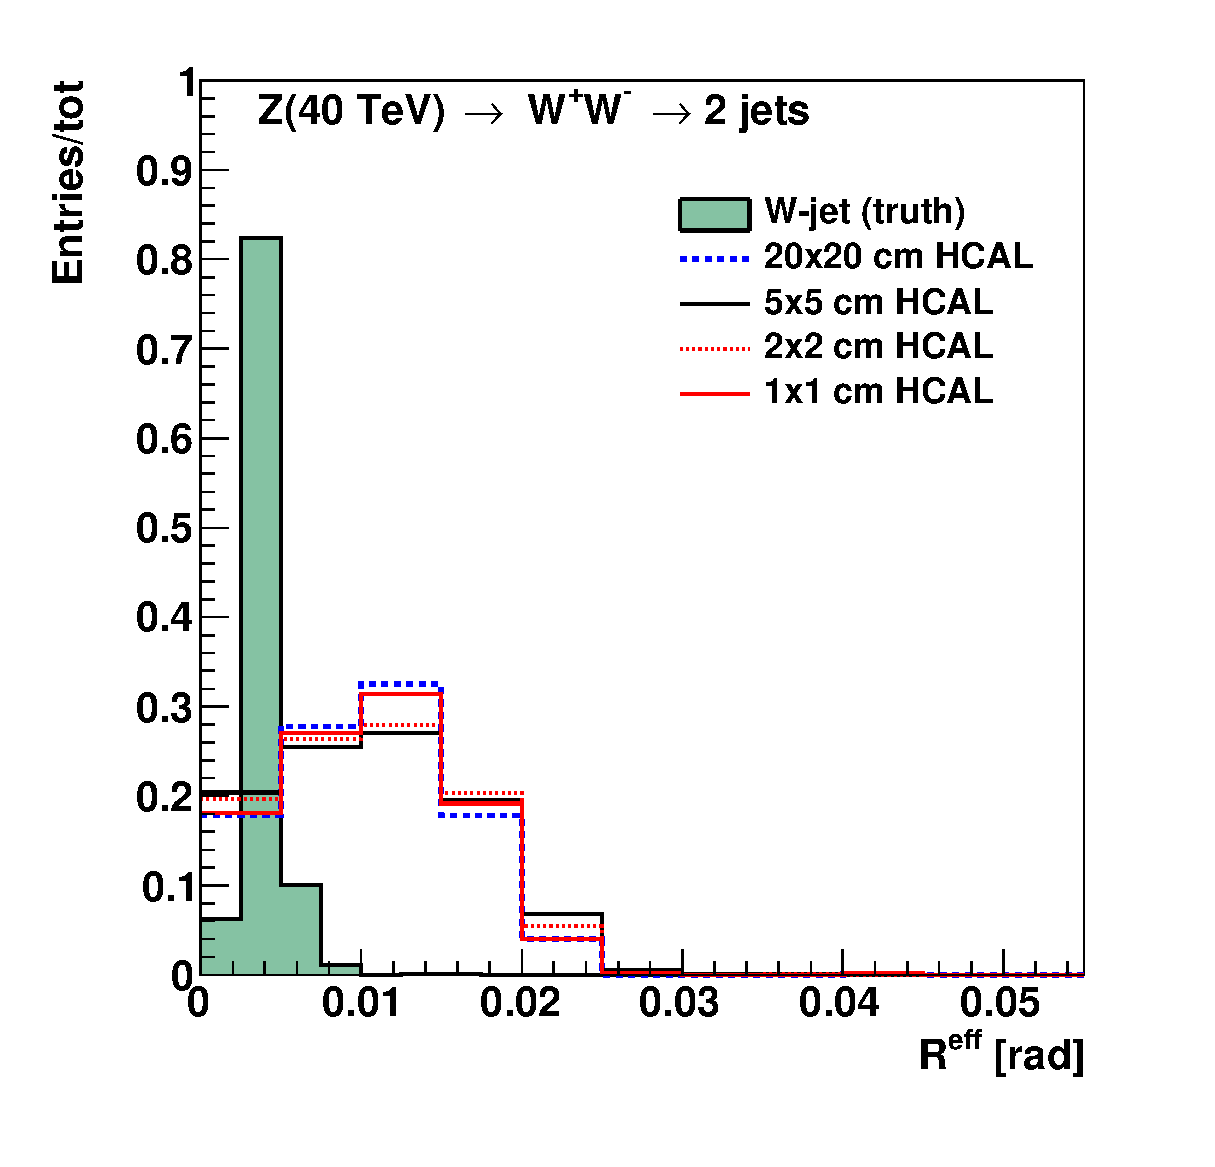
\includegraphics[width=0.43\textwidth]{figs/h40tev_clus_effR_ww1}
   }
\end{center}
\caption{Jet effective radius for different jet transverse moment and HCAL granularity.}
\label{fig:eff_rad}
\end{figure}


Let us study the effect of granularity on jet splitting scales.
A jet $k_T$ splitting scale \cite{Butterworth:2002tt} is defined as a distance measure
used to form jets by the $k_T$ recombination
algorithm \cite{Catani1993187,Ellis:1993tq}.
This has been studied by ATLAS~\cite{ATLAS:2012am}, and more recently in the context of 100 TeV physics \cite{Auerbach:2014xua}.
The distribution of the splitting scale $\sqrt{d_{12}}=\min(p_T^1,p_T^2) \times \delta R_{12}$ \cite{ATLAS:2012am} at the final stage of the $k_T$ clustering, where two subjets are merged into the final one,
is shown in Fig.~\ref{fig:d12}.

\begin{figure}
\begin{center}
   \subfigure[5 TeV] {
   \includegraphics[width=0.43\textwidth]{figs/h5tev_clus_d12_ww1}\hfill
   }
   \subfigure[10 TeV] {
   \includegraphics[width=0.43\textwidth]{figs/h10tev_clus_d12_ww1}
   }
   \subfigure[20 TeV] {
   \includegraphics[width=0.43\textwidth]{figs/h20tev_clus_d12_ww1}
   }
   \subfigure[40 TeV] {
   \includegraphics[width=0.43\textwidth]{figs/h40tev_clus_d12_ww1}
   }
\end{center}
\caption{Jet splitting scale for different jet transverse moment and HCAL granularity.}
\label{fig:d12}
\end{figure}


\subsection{Jet subjettiness}

We recall that $N$-subjettiness~\cite{Ellis:2009su,Thaler:2010tr}, $\tau_{N}$, of jets has been proposed
as a class of variables with which to study the decay products of a heavy particle inside jets.  $\tau_{N}$ is a measure of the degree to which a jet can be considered as being composed of
 $N$  $k_{T}$-subjets \cite{Thaler:2010tr}. 
The variable $\tau_{32}$, defined as the ratio of the $N$-subjettiness variables $\tau_3/\tau_2$, is particularly sensitive to hadronically-decaying
 top-quark initiated jets.
The variable, $\tau_{21} \equiv \tau_2/\tau_1$ can be used to reject background from $W/Z$ decays.
These variables do not strongly correlate with jet mass and can provide an independent check for the
presence of top quarks.
The jet substructure variables were obtained by re-running the $k_T$ algorithm over the jet constituents of anti-$k_T$ jets.

%%%%%%%%%%%%%%% commented out 
\begin{comment}


As an example of the effect of the calorimeter granularity, 
\begin{figure}
\begin{center}
   \subfigure[5 TeV] {
   \includegraphics[width=0.43\textwidth]{figs/r09_tau21b1_20tev_04_U.pdf}\hfill
   }
   \subfigure[10 TeV] {
   \includegraphics[width=0.43\textwidth]{figs/r010_tau21b1_20tev_04_U.pdf}
   }
   \subfigure[20 TeV] {
   \includegraphics[width=0.43\textwidth]{figs/r012_tau21b1_20tev_04_U.pdf}
   }
\end{center}
\caption{Jet subjetinness $\tau_{21}$ for jets originating from splitting scale for different jet transverse moment and HCAL granularity.}
\label{fig:tau21}
\end{figure}


\begin{figure}
\begin{center}
   \subfigure[5 TeV] {
   \includegraphics[width=0.43\textwidth]{figs/r09_tau32b1_20tev_04_U.pdf}\hfill
   }
   \subfigure[10 TeV] {
   \includegraphics[width=0.43\textwidth]{figs/r010_tau32b1_20tev_04_U.pdf}
   }
   \subfigure[20 TeV] {
   \includegraphics[width=0.43\textwidth]{figs/r012_tau32b1_20tev_04_U.pdf}
   }
\end{center}
\caption{Jet subjetinness $\tau_{32}$ for jets originating from splitting scale for different jet transverse moment and HCAL granularity.}
\label{fig:tau21}
\end{figure}

%%%%%%%%%%%%%%% commented out 
\end{comment}



\section{Study of detector performance with soft drop mass}
In this section, we use the jet mass computed with a specific algorithm, soft 
drop declustering, to study the performance of detector with various detector 
cell sizes and center-of-mass (c.m.) energies. 
\subsection{The technique of soft drop declustering}
The soft drop declustering~\cite{Larkoski:2014wba} is a grooming method 
that removes soft wide-angle radiation from a jet. The constituents of a jet 
$j_0$ are first reclustered using the Cambridge-Aachen
 (C/A) algorithm~\cite{Dokshitzer:1997in,Wobisch:1998wt}. Then, the jet $j_0$ 
is broken into two subjets $j_1$ and $j_2$ by undoing the last stage of C/A 
clustering.
If the subjets pass the following soft drop condition, jet $j_0$ is the final 
soft-drop jet. Otherwise, the algorithm redefines $j_0$ to be the subjet with 
larger $p_T$ (among $j_1$ and $j_2$) and iterates the procedure.
\begin{equation} \label{eq:soft-drop}
\frac{\mathrm{min}(p_{T1},p_{T2})}{p_{T1}+p_{T2}}>z_\mathrm{cut}(\frac{\Delta R_{12}}{R_{0}})^{\beta},
\end{equation}
where $p_{T1}$ and $p_{T2}$ are the transverse momenta of the two subjets, 
$z_\mathrm{cut}$ is soft drop threshold, 
$\Delta R_{12}$ is the distance between the two subjets in the $\eta$-$\phi$ 
plane, $R_0$ is the characteristic radius of the original jet, and $\beta$ is 
the angular exponent.

In our study, we compare the performance of future detector when setting 
$\beta=0$ versus when setting $\beta=2$. For $\beta=0$, the soft drop condition 
depends only on the $z_\mathrm{cut}$. For $\beta=2$, the condition depends on 
the angular distance between the two subjets and $z_\mathrm{cut}$ and the 
algorithm becomes infrared and collinear safe. 

\subsection{Analysis method}
We employ the following method to quantify the detector performance and 
find out the cell size that gives the best separation power to distinguish 
signal from background. For each configuration of detector and c.m. energy, 
we draw the receiver operating characteristic (ROC) curves in which the x-axis
 is the signal efficiency ($\epsilon_\mathrm{sig}$) and y-axis is the inverse 
of background efficiency ($1/\epsilon_\mathrm{bkg}$). 
In order to scan the efficiencies of soft drop mass cuts, we vary the mass 
window as follows. We first look for the median bin 
$i_\mathrm{med}$\footnote{The integral from bin 0 to bin $i_\mathrm{med}$ 
($i_\mathrm{med}-1$) should be greater (less) than half 
of the total number of events. Note, the bin width is 5~GeV.} of the soft 
drop mass histogram from simulated signal events. Taking the right boundary
 of bin $i_\mathrm{med}$ as the center of mass window 
$x_\mathrm{center}$, we start increasing the width of mass window symmetrically
 on the left and on the right of $x_\mathrm{center}$, in steps of 5~GeV, 
i.e. the narrowest mass window is 
[$x_\mathrm{center}-5,x_\mathrm{center}+5$]. If one side reaches the boundary 
of the mass histogram, we only increase the width on the other side, also in 
steps of 5~GeV. For each mass window, there will be corresponding 
$\epsilon_\mathrm{sig}$ and $\epsilon_\mathrm{bkg}$, which gives a point in 
the ROC curves.

\subsection{Results and conclusion}
Figures~\ref{fig:cluster_mass_mmdt_ww}, \ref{fig:cluster_mass_mmdt_tt},
 \ref{fig:cluster_mass_sdb2_ww}, and \ref{fig:cluster_mass_sdb2_tt} 
present the distributions of soft drop mass for $\beta=0$ and $\beta=2$ with 
different c.m. energies and detector cell sizes; the signals considered are 
Z'$\rightarrow$WW and Z'$\rightarrow$t$\bar{\mathrm{t}}$. 
In Figs.~\ref{fig:cluster_mass_mmdt_ww_ROC}, \ref{fig:cluster_mass_mmdt_tt_ROC}, \ref{fig:cluster_mass_sdb2_ww_ROC}, and \ref{fig:cluster_mass_sdb2_tt_ROC}, 
ROC curves from different detector cell sizes are compared for each 
c.m. energy, respectively. 

Figures~\ref{fig:cluster_mass_mmdt_ww_ROC} and 
\ref{fig:cluster_mass_mmdt_tt_ROC} show that for $\beta=0$ the 
smallest detector cell size, 
 $1~\mathrm{cm}\times1~\mathrm{cm}$, has the best separation power at 
$\sqrt{s}=$5, 10, and 20 TeV when the signal is Z'$\rightarrow$WW and 
at  $\sqrt{s}=$10 and 20 TeV when the signal is Z'$\rightarrow$t$\bar{\mathrm{t}}$.
On the contrary, Figs.~\ref{fig:cluster_mass_sdb2_ww_ROC} and \ref{fig:cluster_mass_sdb2_tt_ROC} show that for $\beta=2$ the smallest detector cell size 
does not have improvements in the separation power with respect to those with 
larger cell sizes. In fact, the performances of the three cell sizes are 
similar. In addition, sometimes bigger detector cell sizes, 
$5~\mathrm{cm}\times5~\mathrm{cm}$ or $20~\mathrm{cm}\times20~\mathrm{cm}$
 have the best separation power. 

We also find compared to $\beta=2$, soft drop mass with $\beta=0$ has better 
performance for distinguishing signal from background. Therefore, we will 
apply requirements on this variable when studying the other jet substructure 
variables. 
 
%50bins
\begin{figure}
\begin{center}
   \subfigure[20$\times$20($cm^2$)] {
   \includegraphics[ width=0.3\textwidth]{h_soft_drop/Dis_cluster_010_mass_mmdt_20tev_04_no_UOF.eps}
   }
      \subfigure[5$\times$5($cm^2$)] {
   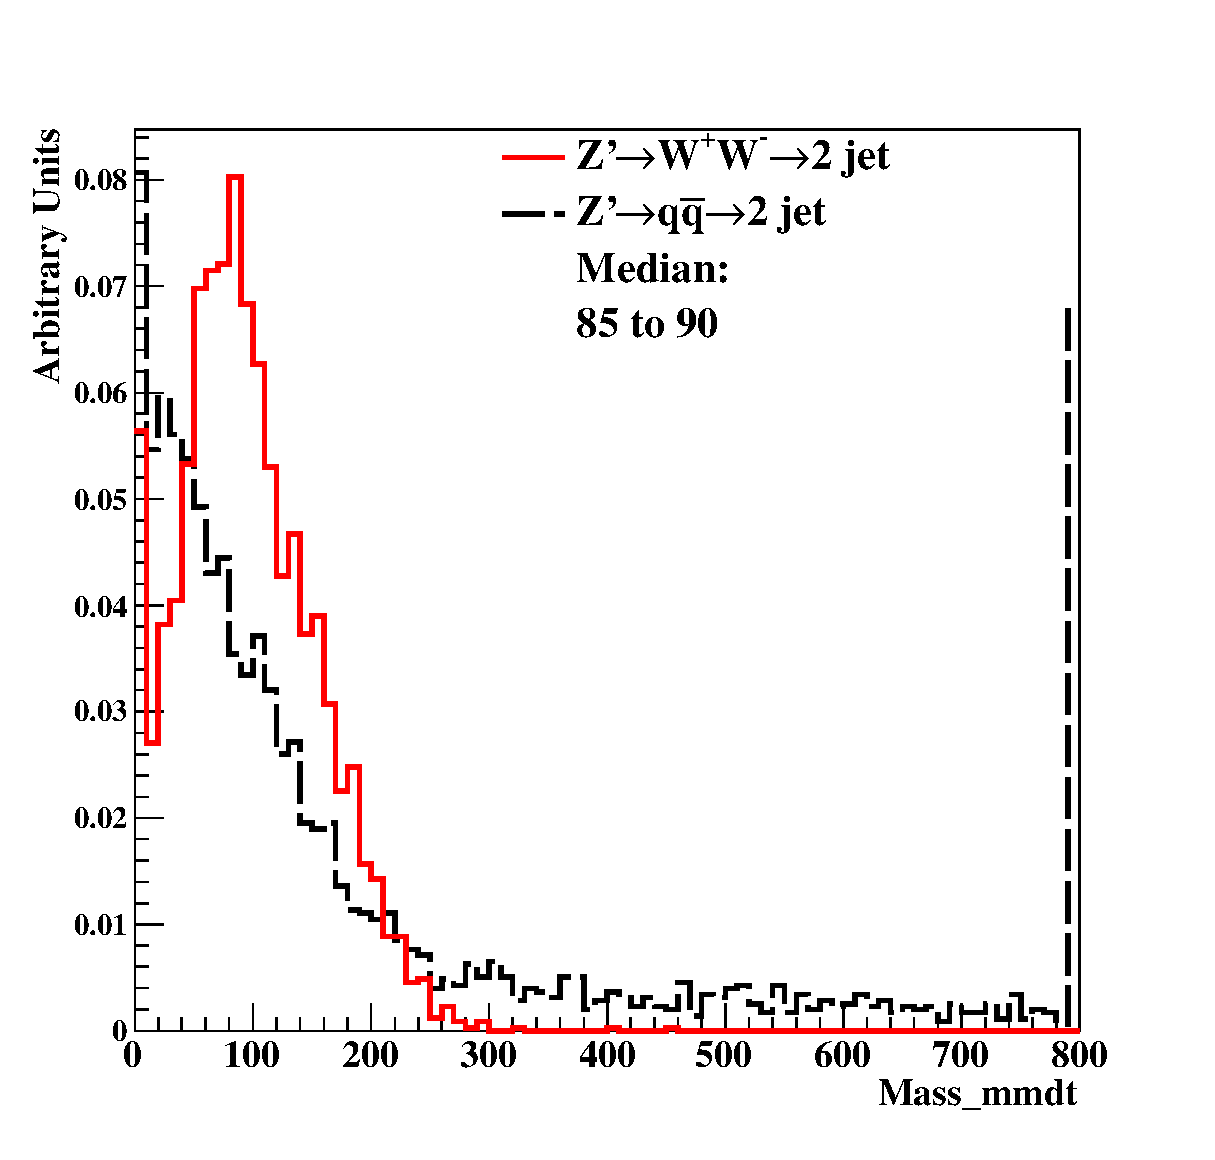
\includegraphics[ width=0.3\textwidth]{h_soft_drop/Dis_cluster_009_mass_mmdt_20tev_04_no_UOF.eps}\hfill
   }
   \subfigure[1$\times$1($cm^2$)] {
   \includegraphics[ width=0.3\textwidth]{h_soft_drop/Dis_cluster_012_mass_mmdt_20tev_04_no_UOF.eps}\hfill
   }
\end{center}
\caption{Distributions of soft drop mass for $\beta$=0, with 20 TeV c.m. energies and three different detector cell sizes: 20$\times$20, 
5$\times$5, and 1$\times$1 ($cm^2$). The signal (background) process is 
Z'$\rightarrow$WW (Z'$\rightarrow$q$\bar{\mathrm{q}}$).
\label{fig:cluster_mass_mmdt_ww}}
\end{figure}


\begin{figure}
\begin{center}
  \subfigure[Z'(5 TeV)] {
  \includegraphics[  width=0.45\textwidth]{ROC_soft_drop/A_Cluster_mass_mmdt_5tev_eff_1_central_fix_at_Median_bin_ww_qq_log_no_UOF.eps}
  }
  \subfigure[Z'(10 TeV)] {
  \includegraphics[  width=0.45\textwidth]{ROC_soft_drop/A_Cluster_mass_mmdt_10tev_eff_1_central_fix_at_Median_bin_ww_qq_log_no_UOF.eps}
  }
 \subfigure[Z'(20 TeV)] {
 \includegraphics[  width=0.45\textwidth]{ROC_soft_drop/A_Cluster_mass_mmdt_20tev_eff_1_central_fix_at_Median_bin_ww_qq_log_no_UOF.eps}
 }
 \subfigure[Z'(40 TeV)] {
 \includegraphics[  width=0.45\textwidth]{ROC_soft_drop/A_Cluster_mass_mmdt_40tev_eff_1_central_fix_at_Median_bin_ww_qq_log_no_UOF.eps}
 }
\end{center}
\caption{The ROC curves of soft drop mass selection for $\beta$=0 
with 5, 10, 20, 40 TeV c.m. energies. 
Three different detector cell sizes are compared: 20$\times$20, 
5$\times$5, and 1$\times$1 ($cm^2$). 
The signal (background) process is Z'$\rightarrow$WW 
(Z'$\rightarrow$q$\bar{\mathrm{q}}$).}
\label{fig:cluster_mass_mmdt_ww_ROC}
\end{figure}


\begin{figure}
\begin{center}
   \subfigure[5$\times$5 ($cm^2$)] {
   \includegraphics[   width=0.3\textwidth]{h_soft_drop/Dis_cluster_010_mass_mmdt_tt_20tev_04_tt_no_UOF.eps}
   }
   \subfigure[20$\times$20 ($cm^2$)] {
   \includegraphics[   width=0.3\textwidth]{h_soft_drop/Dis_cluster_009_mass_mmdt_tt_20tev_04_tt_no_UOF.eps}\hfill
   }
   \subfigure[1$\times$1 ($cm^2$)] {
   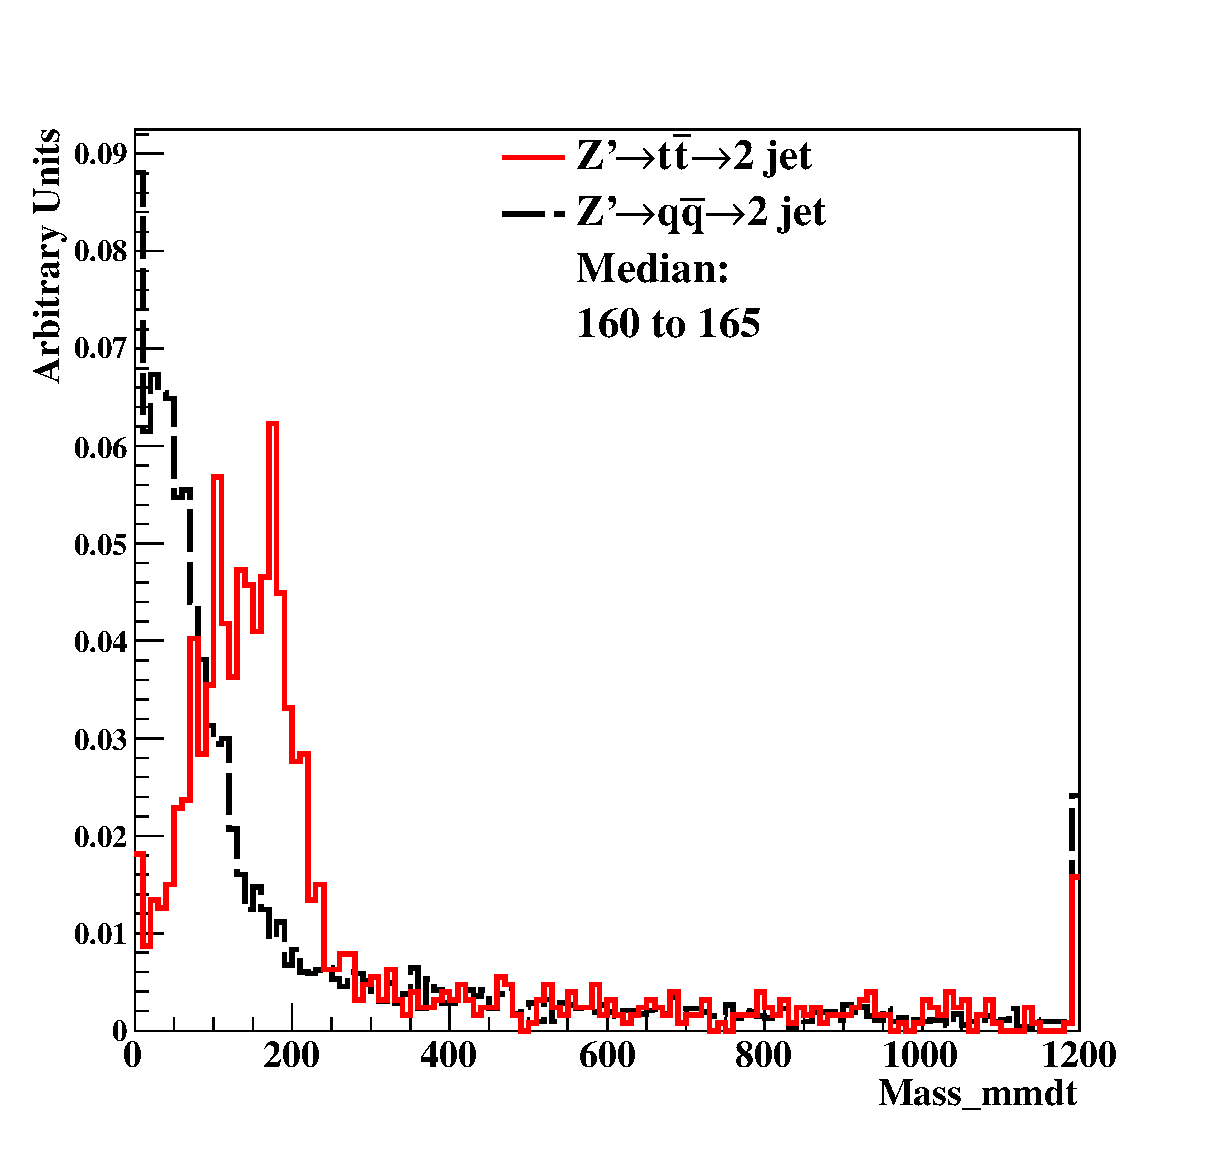
\includegraphics[   width=0.3\textwidth]{h_soft_drop/Dis_cluster_012_mass_mmdt_tt_20tev_04_tt_no_UOF.eps}\hfill
   }
\end{center}
\caption{
Distributions of soft drop mass for $\beta$=0, with 20 TeV c.m. energies and three different detector cell sizes: 20$\times$20, 
5$\times$5, and 1$\times$1 ($cm^2$). The signal (background) process is 
Z'$\rightarrow$t$\bar{\mathrm{t}}$ (Z'$\rightarrow$q$\bar{\mathrm{q}}$).
}
\label{fig:cluster_mass_mmdt_tt}
\end{figure}


\begin{figure}
\begin{center}
  \subfigure[Z'(5 TeV)] {
  \includegraphics[  width=0.45\textwidth]{ROC_soft_drop/A_Cluster_mass_mmdt_5tev_eff_1_central_fix_at_Median_bin_tt_qq_log_no_UOF.eps}
  }
  \subfigure[Z'(10 TeV)] {
  \includegraphics[  width=0.45\textwidth]{ROC_soft_drop/A_Cluster_mass_mmdt_10tev_eff_1_central_fix_at_Median_bin_tt_qq_log_no_UOF.eps}
  }
 \subfigure[Z'(20 TeV)] {
 \includegraphics[  width=0.45\textwidth]{ROC_soft_drop/A_Cluster_mass_mmdt_20tev_eff_1_central_fix_at_Median_bin_tt_qq_log_no_UOF.eps}
 }
 \subfigure[Z'(40 TeV)] {
 \includegraphics[  width=0.45\textwidth]{ROC_soft_drop/A_Cluster_mass_mmdt_40tev_eff_1_central_fix_at_Median_bin_tt_qq_log_no_UOF.eps}
 }
\end{center}
\caption{
The ROC curves of soft drop mass selection for $\beta$=0 
with 5,10, 20, 40 TeV c.m. energies. 
Three different detector cell sizes are compared: 20$\times$20, 
5$\times$5, and 1$\times$1 ($cm^2$). 
The signal (background) process is Z'$\rightarrow$t$\bar{\mathrm{t}}$
(Z'$\rightarrow$q$\bar{\mathrm{q}}$).
}
\label{fig:cluster_mass_mmdt_tt_ROC}
\end{figure}



\begin{figure}
\begin{center}
   \subfigure[20$\times$20 ($cm^2$)] {
   \includegraphics[   width=0.3\textwidth]{h_soft_drop/Dis_cluster_010_mass_sdb2_ww_20tev_04_1600_no_UOF.eps}
   }
    \subfigure[5$\times$5 ($cm^2$)] {
   \includegraphics[   width=0.3\textwidth]{h_soft_drop/Dis_cluster_009_mass_sdb2_ww_20tev_04_1600_no_UOF.eps}\hfill
   }
   \subfigure[1$\times$1 ($cm^2$)] {
   \includegraphics[   width=0.3\textwidth]{h_soft_drop/Dis_cluster_012_mass_sdb2_ww_20tev_04_1600_no_UOF.eps}\hfill
   }
\end{center}
\caption{
Distributions of soft drop mass for $\beta$=2, with 20 TeV c.m. energies and three different detector cell sizes: 20$\times$20, 
5$\times$5, and 1$\times$1 ($cm^2$). The signal (background) process is 
Z'$\rightarrow$WW (Z'$\rightarrow$q$\bar{\mathrm{q}}$).
}
\label{fig:cluster_mass_sdb2_ww}
\end{figure}


\begin{figure}
\begin{center}
  \subfigure[Z'(5 TeV)] {
  \includegraphics[  width=0.45\textwidth]{ROC_soft_drop/A_Cluster_mass_sdb2_5tev_eff_1_central_fix_at_Median_bin_ww_qq_log_no_UOF.eps}
  }
  \subfigure[Z'(10 TeV)] {
  \includegraphics[  width=0.45\textwidth]{ROC_soft_drop/A_Cluster_mass_sdb2_10tev_eff_1_central_fix_at_Median_bin_ww_qq_log_no_UOF.eps}
  }
 \subfigure[Z'(20 TeV)] {
 \includegraphics[  width=0.45\textwidth]{ROC_soft_drop/A_Cluster_mass_sdb2_20tev_eff_1_central_fix_at_Median_bin_ww_qq_log_no_UOF.eps}
 }
 \subfigure[Z'(40 TeV)] {
 \includegraphics[  width=0.45\textwidth]{ROC_soft_drop/A_Cluster_mass_sdb2_40tev_eff_1_central_fix_at_Median_bin_ww_qq_log_no_UOF.eps}
 }
\end{center}
\caption{
The ROC curves of soft drop mass selection for $\beta$=2
with 5, 10, 20, 40 TeV c.m. energies. 
Three different detector cell sizes are compared: 20$\times$20, 
5$\times$5, and 1$\times$1 ($cm^2$). 
The signal (background) process is Z'$\rightarrow$WW 
(Z'$\rightarrow$q$\bar{\mathrm{q}}$).
}
\label{fig:cluster_mass_sdb2_ww_ROC}
\end{figure}


\begin{figure}
\begin{center}
   \subfigure[20$\times$20 ($cm^2$)] {
   \includegraphics[   width=0.3\textwidth]{h_soft_drop/Dis_cluster_010_mass_sdb2_tt_20tev_04_tt_2400_no_UOF.eps}
   }
   \subfigure[5$\times$5 ($cm^2$)] {
   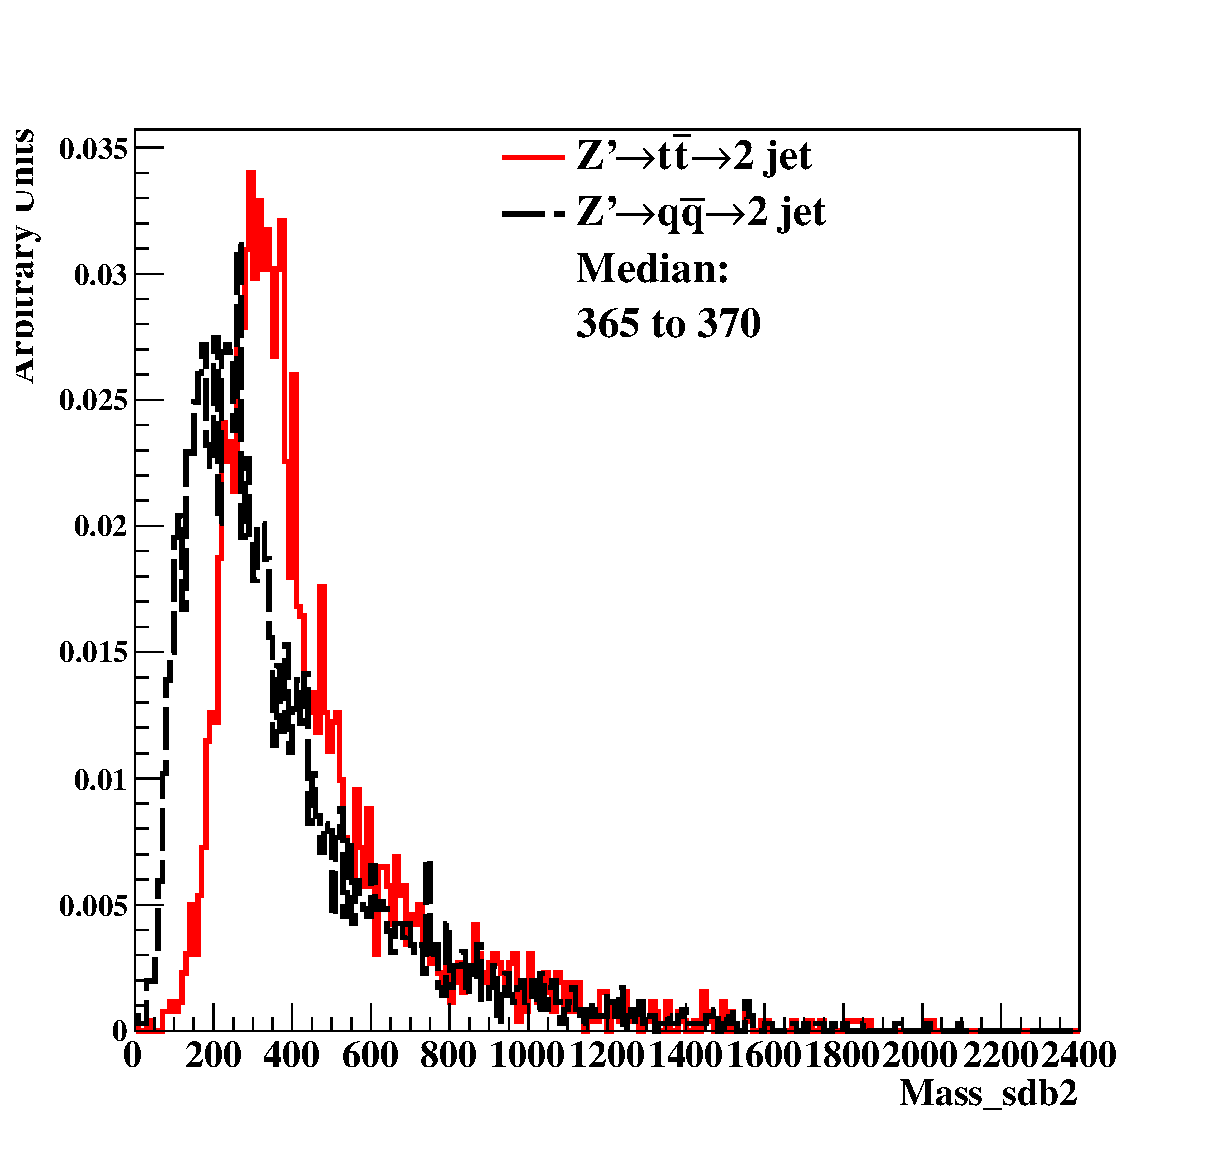
\includegraphics[   width=0.3\textwidth]{h_soft_drop/Dis_cluster_009_mass_sdb2_tt_20tev_04_tt_2400_no_UOF.eps}\hfill
   }
   \subfigure[1$\times$1 ($cm^2$)] {
   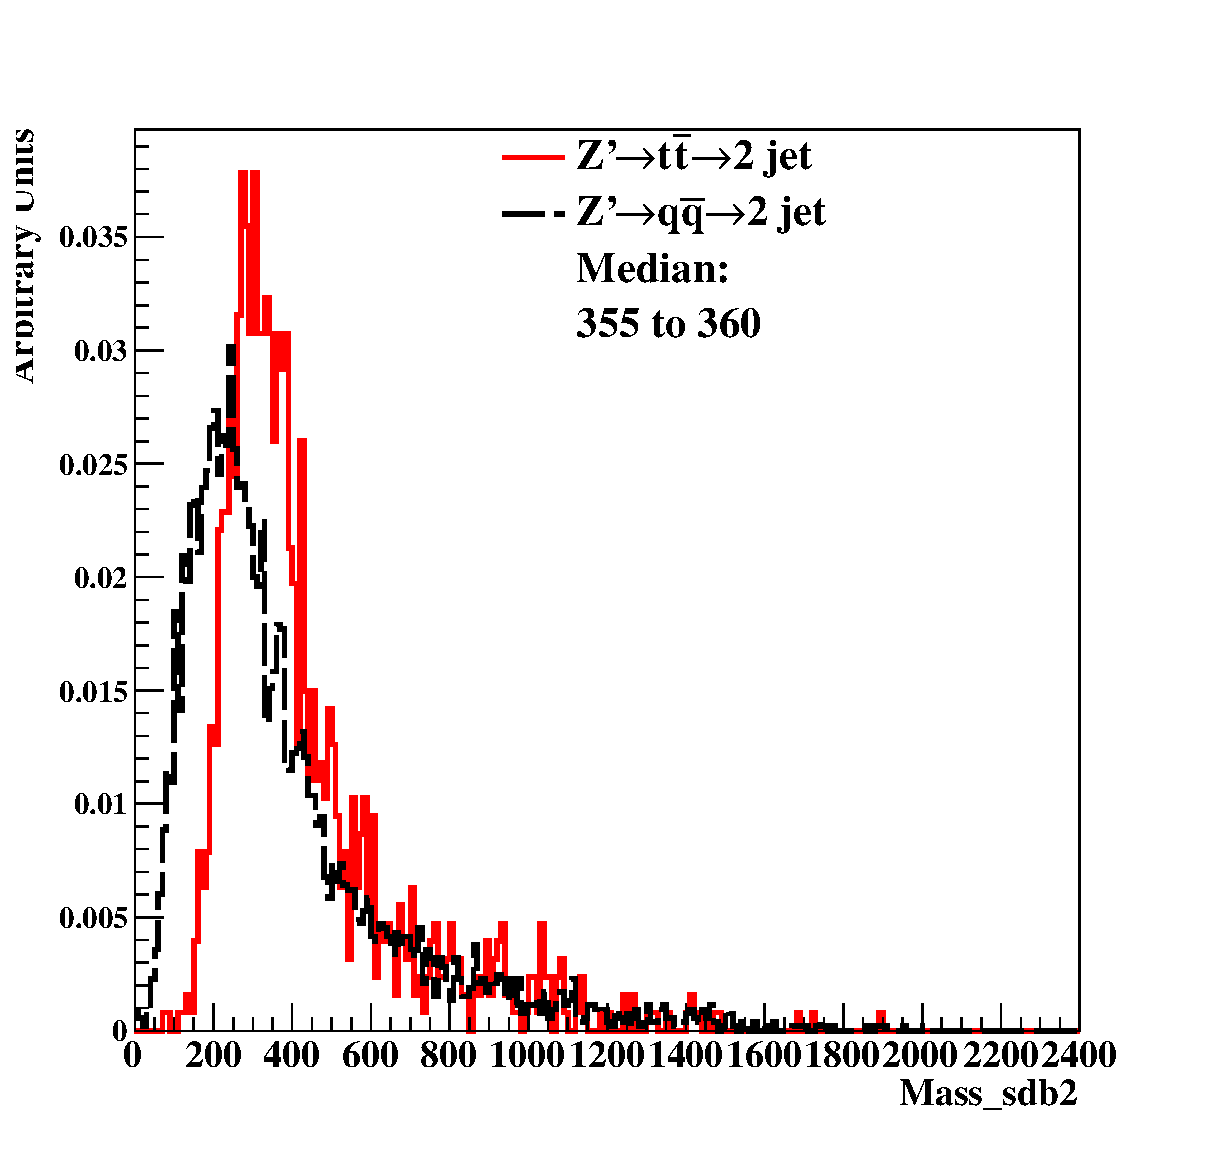
\includegraphics[   width=0.3\textwidth]{h_soft_drop/Dis_cluster_012_mass_sdb2_tt_20tev_04_tt_2400_no_UOF.eps}\hfill
   }
\end{center}
\caption{
Distributions of soft drop mass for $\beta$=2, with 20 TeV c.m. energies and three different detector cell sizes: 20$\times$20, 
5$\times$5, and 1$\times$1 ($cm^2$). The signal (background) process is 
Z'$\rightarrow$t$\bar{\mathrm{t}}$ (Z'$\rightarrow$q$\bar{\mathrm{q}}$).
}
\label{fig:cluster_mass_sdb2_tt}
\end{figure}


\begin{figure}
\begin{center}
  \subfigure[Z'(5 TeV)] {
  \includegraphics[  width=0.45\textwidth]{ROC_soft_drop/A_Cluster_mass_sdb2_5tev_eff_1_central_fix_at_Median_bin_tt_qq_log_no_UOF.eps}
  }
  \subfigure[Z'(10 TeV)] {
  \includegraphics[  width=0.45\textwidth]{ROC_soft_drop/A_Cluster_mass_sdb2_10tev_eff_1_central_fix_at_Median_bin_tt_qq_log_no_UOF.eps}
  }
 \subfigure[Z'(20 TeV)] {
 \includegraphics[  width=0.45\textwidth]{ROC_soft_drop/A_Cluster_mass_sdb2_20tev_eff_1_central_fix_at_Median_bin_tt_qq_log_no_UOF.eps}
 }
 \subfigure[Z'(40 TeV)] {
 \includegraphics[  width=0.45\textwidth]{ROC_soft_drop/A_Cluster_mass_sdb2_40tev_eff_1_central_fix_at_Median_bin_tt_qq_log_no_UOF.eps}
 }
\end{center}
\caption{
The ROC curves of soft drop mass selection for $\beta$=2
with 5, 10, 20, 40 TeV c.m. energies. 
Three different detector cell sizes are compared: 20$\times$20, 
5$\times$5, and 1$\times$1 ($cm^2$). 
The signal (background) process is Z'$\rightarrow$t$\bar{\mathrm{t}}$
(Z'$\rightarrow$q$\bar{\mathrm{q}}$).
}
\label{fig:cluster_mass_sdb2_tt_ROC}
\end{figure}






\section{Studies of signal and background separation using jet substructure variables}
In this section, we study different jet substructure variables and compare their ability to separate signal from background with different detector sizes and c.m. energy using Mann-Whitney U test and ROC curves.\\

By definition of Mann Whitney U test, if U value is close to 0.5, it means two distributions have similar compositions, and we can not distinguish them very well. On the other hand, if U value of two distributions are close to 0, it means both compositions of both distribution are much different from each other.\\

\subsection{N-subjettiness}
N-subjettiness[\ref{}] is the detection technique of jet substructure that is used to identify boosted hadronically-decaying objects under the high c.m. conditions. We use $\tau$ variable to distinguish the number of subjet in a fatjet to separate signal and background with different detector sizes and c.m. energy.\\

\subsubsection{The technic of N-subjettiness}
The formula and the technique are as following:\\
\begin{equation}\label{eq:Nsub_1}
\tau_{N}=\frac{1}{d_{0}}\sum_{k}p_{T,k} min\{\Delta R_{1,k},\Delta R_{2,k},.....\Delta R_{N,k}\}
\end{equation}
\begin{equation}
d_{0}=\sum_{k}p_{T,k} R_{0}
\end{equation}
k runs over all constituent particles in the given jets (fatjet), $p_{T,k}$ are their transverse momentum, $\Delta R_{J,k}=\sqrt{(\Delta \eta)^{2}+(\Delta \phi)^{2}}$ is the distance between the constituent particles k and the candidate subjet J on the $\eta-\phi$ plane. $R_{0}$ is the characteristic jet radius used in Anti-kt(AK) jet algorithm at starting. $d_{0}$ is the normalization factor.\\
\begin{enumerate}
\item First, Anti-kt(AK) algorithm is used to reconstruct jets
\item Second, after reconstructing the AK4 jets, exclusive $k_{T}$ algorithm[\ref{}] is used in finding the jet axis in a fatjet.
\item Third, start running formula [\ref{eq:Nsub_1}] and loop all constituent particles in a fatjet.
\item Finally, when finishing running all particles, it will give out $\tau_{N}$, where N is positive integer. 
\end{enumerate}

If a fatjet has N subjet(s)[\ref{}], its $\tau_{N}$ is smaller than the $\tau_{N}$ of the fatjet with different number of subjets. For example, if we compare the  $\tau_{2}$ of one-subjet fatjet and two-subjets one, two-subjets fatjet has smaller $\tau_{2}$ than one-subjet one. On the other hand, one-subjet fatjet has smaller $\tau_{1}$ than two-subjets one. In the end, we can use the ratio of  $\tau_{2}$ and  $\tau_{1}$ ( $\tau_{21}$) to distinguish fatjet with one-subjet case and-two subjets case.$\tau_{21}$ is used to discriminate the fatjet shape, and it can be modified with different number of subjet.\\

In our study, we use $\tau_{21}$  and $\tau_{32}$ in distinguishing two-subjets fatjet and three-subjets fatjet from one-subjet fatjet individually. We want to use this two ratio values to distinguish signal from background.\\
\subsubsection{Analysis method}
First, we select the events in mass window by using SD with $\beta=0$ and 75$\%$ signal efficiency. Then, we find the highest ratio bin to be our seed bin. Next, we compare the left and right of ratio bin, and add the higher bin to be our width. Finally,  We can use this width to draw the ROC curves.\\2
\subsubsection{The results and conclusion}
In the figure [\ref{fig:Rawhit_05GeV_tau21_Dis}][\ref{fig:Rawhit_05GeV_tau32_Dis}], they show the histograms of $\tau_{21}$ and $\tau_{32}$ after selecting the events. In all figures, they also include the Mann-Whitney U value in ir the legend.\\

As a result of figure [\ref{fig:Rawhit_05GeV_tau21_ROC}][\ref{fig:Rawhit_05GeV_tau32_ROC}], they perform the ROC curves of $\tau_{21}$ and $\tau_{32}$ with different detector cell sizes and c.m. energy. The smallest detector cell (1$\times$1) doesn't have the best separation power to distinguish signal from background. Some of them have the best separation power with the bigger cell size (5$\times$5 and 20$\times$20).\\

In Figure [\ref{fig:Rawhit_05GeV_total_Mann}](a)(b), they show the summary plots of $\tau_{21}$ and $\tau_{32}$ with the rawhit cut with 0.5GeV using Mann Whitney U test. In $\tau_{21}$, 5TeV has better separation power when detector sizes get smaller. When energy increases, there is no improvement in the smallest detector cell size (1$\times$1). In $\tau_{32}$, the case is similar to  $\tau_{21}$. Even worse, with some c.m. energies, the bigger detector sizes (5$\times$5 and 20$\times$20) have better separation power than the smallest detector sizes (1$\times$1). 
\subsection{Studies of signal and background separation using jet substurcture variable: Energy correlation function}
Energy correlation function (ECF) [\ref{}] is another kind of detection technique of jet substurcture that is used to distinguish the number of subjets in a fatjet under high c.m. energy conditions. This method only uses the momenta of particles and the angles between them without additional algorithm.\\
\subsubsection{The technic of energy correlation function}
The basic ECF formula is as following:\\
\begin{equation} \label{eq:ECF_Original}
ECF(N,\beta)=\sum_{i_{1}<i_{2}<....<i_{N}\in J} (\prod_{a=1}^{N}E_{ia})(\prod_{b=1}^{N-1}\prod_{c=b+1}^{N} \theta_{i_{b}i_{c}})^{\beta}
\end{equation}

In the formula \ref{eq:ECF_Original}, the sum loop all particles in the jet $J$, $E$ are the energy of particles, and $\theta$ are the angles between the particles.

We apply two approximation. First, because under the high energy limitation $p>>m$, $E\approx p$. Second, we use Radius R between particles naturally, so our ECF formula (\ref{eq:ECF_Original}) can be modified to the formula:\\  
\begin{equation} \label{eq:ECF_Modified}
ECF(N,\beta)=\sum_{i_{1}<i_{2}<....<i_{N}\in J} (\prod_{a=1}^{N}P_{ia})(\prod_{b=1}^{N-1}\prod_{c=b+1}^{N} R_{i_{b}i_{c}})^{\beta}
\end{equation}

From the modified ECF formula (\ref{eq:ECF_Modified}), in order to use the dimensionless observation to determine whether the number of subjets in system, parameter $\tau_{N}$ is defined as:\\
\begin{equation} \label{eq:ECF_ratio}
\tau_{N}^{(\beta)}\equiv\frac{ECF(N+1,\beta)}{ECF(N,\beta)}
\end{equation}

The idea of formula (\ref{eq:ECF_ratio}) is from N-subjetness, because the behavior of it is very similar to N-subjetness as reference [\ref{}]. In general, if the system has N subjets, $ECF(N+1,\beta)$ should be significantly smaller than $ECF(N,\beta)$, so we can use this advantage to distinguish different number of subjets. FInally, because it is suggested to used $\tau_{21}$, $\tau_{32}$ [\ref{}] to distinguish two-subjets fatjet and three-subjets fatjet from one-subjet fatjet, in the ECF, it also defines the ratio of $\tau$ there, and define the energy correlation double ratio that is used in our study:\\
\begin{equation}
C_{N}^{(\beta)}\equiv\frac{\tau_{N}^{(\beta)}}{\tau_{N-1}^{(\beta)}}=\frac{ECF(N-1,\beta)ECF(N+1,\beta)}{ECF(N,\beta)^2}
\end{equation}

We set N=2 and $\beta=1$ ($C_{2}^{1}$) to distinguish two-subjets fatjet from one-subjet fatjet.
\subsubsection{Analysis method}
First, we select the events in mass window by using SD with $\beta=0$ and 75$\%$ signal efficiency. Then, we find the highest ratio bin to be our seed bin. Next, we compare the left and right of ratio bin, and add the higher bin to be our width. Finally,  We can use this width to draw the ROC curves.\\
\subsubsection{The results and conclusion}
In the figure [\ref{fig:Rawhit_05GeV_c2b1_Dis}], they show the histograms of $\tau_{21}$ and $\tau_{32}$ after selecting the events. In all figures, they also include the Mann-Whitney U value in their legend\\

As a result of figure [\ref{fig:Rawhit_05GeV_c2b1_ROC}], they perform the ROC curves of $C_{2}^{1}$ with different detector cell sizes and c.m. energy. The smallest detector cell (1$\times$1) doesn't have the best separation power to distinguish signal from background. In addition, in some cases such like (a), the biggest one (20$\times$20) has the best distinguish power under the same c.m. energy.\\

In Figure [\ref{fig:Rawhit_05GeV_total_Mann}](c), it shows the summary plots with the rawhit cut with 0.5GeV using Mann Whitney U test. For conclusion, all separation power aren't improved by smallest cell size (1$\times$1).\\

%25bins
\begin{figure}
\begin{center}
   \subfigure[20$\times$20($cm^2$)] {
   \includegraphics[width=0.43\textwidth]{h_Tau_C/Dis_Rawhit_05GeV_010_c2b1_20tev_04_after_cut_Man_25_no_UOF_new_75pa_for_paper.eps}
   }
   \subfigure[5$\times$5($cm^2$)] {
   \includegraphics[width=0.43\textwidth]{h_Tau_C/Dis_Rawhit_05GeV_009_c2b1_20tev_04_after_cut_Man_25_no_UOF_new_75pa_for_paper.eps}
   }
   \subfigure[$\times$1($cm^2$)] {
   \includegraphics[width=0.43\textwidth]{h_Tau_C/Dis_Rawhit_05GeV_012_c2b1_20tev_04_after_cut_Man_25_no_UOF_new_75pa_for_paper.eps}
   }
\end{center}
\caption{Distributions of Mann-Whitney value U in 20 TeV energy collision for c2b1 in different detector sizes. Cell Size in 20$\times$20, 5$\times$5, and 1$\times$1(cm$\times$cm) are shown here.}
\label{fig:Rawhit_05GeV_c2b1_Dis}
\end{figure}

\begin{figure}
\begin{center}
   \subfigure[Z'(5 TeV)] {
   \includegraphics[width=0.43\textwidth]{ROC_Tau_C/Rawhit_05GeV_c2b1_5tev_eff_1_New2_after_cut_25bins_no_UOF_new_75pa.eps}\hfill
   }
   \subfigure[Z'(10 TeV)] {
   \includegraphics[width=0.43\textwidth]{ROC_Tau_C/Rawhit_05GeV_c2b1_10tev_eff_1_New2_after_cut_25bins_no_UOF_new_75pa.eps}
   }
   \subfigure[Z'(20 TeV)] {
   \includegraphics[width=0.43\textwidth]{ROC_Tau_C/Rawhit_05GeV_c2b1_20tev_eff_1_New2_after_cut_25bins_no_UOF_new_75pa.eps}
   }
   \subfigure[Z'(40 TeV)] {
   \includegraphics[width=0.43\textwidth]{ROC_Tau_C/Rawhit_05GeV_c2b1_40tev_eff_1_New2_after_cut_25bins_no_UOF_new_75pa.eps}
   }
\end{center}
\caption{Signal efficiency versus background rejection rate using c2b1.The energies of collision at (a)5, (b)10, (c)20, (d)40TeV are shown here. In each picture, the three ROC curves correspond to different detector sizes.}
\label{fig:Rawhit_05GeV_c2b1_ROC}
\end{figure}



%25bins
\begin{figure}
\begin{center}
   \subfigure[20$\times$20($cm^2$)] {
   \includegraphics[width=0.43\textwidth]{h_Tau_C/Dis_Rawhit_05GeV_010_tau21_20tev_04_after_cut_Man_25_no_UOF_new_75pa_for_paper.eps}
   }
   \subfigure[5$\times$5($cm^2$)] {
   \includegraphics[width=0.43\textwidth]{h_Tau_C/Dis_Rawhit_05GeV_009_tau21_20tev_04_after_cut_Man_25_no_UOF_new_75pa_for_paper.eps}
   }
   \subfigure[1$\times$1($cm^2$)] {
   \includegraphics[width=0.43\textwidth]{h_Tau_C/Dis_Rawhit_05GeV_012_tau21_20tev_04_after_cut_Man_25_no_UOF_new_75pa_for_paper.eps}
   }
\end{center}
\caption{Distributions of Mann-Whitney value U in 20 TeV energy collision for $\tau_{21}$  in different detector sizes. Cell Size in 20$\times$20, 5$\times$5, and 1$\times$1(cm$\times$cm) are shown here.}
\label{fig:Rawhit_05GeV_tau21_Dis}
\end{figure}

\begin{figure}
\begin{center}
   \subfigure[Z'(5 TeV)] {
   \includegraphics[width=0.43\textwidth]{ROC_Tau_C/Rawhit_05GeV_tau21_5tev_eff_1_New2_after_cut_25bins_no_UOF_new_75pa.eps}\hfill
   }
   \subfigure[Z'(10 TeV)] {
   \includegraphics[width=0.43\textwidth]{ROC_Tau_C/Rawhit_05GeV_tau21_10tev_eff_1_New2_after_cut_25bins_no_UOF_new_75pa.eps}
   }
   \subfigure[Z'(20 TeV)] {
   \includegraphics[width=0.43\textwidth]{ROC_Tau_C/Rawhit_05GeV_tau21_20tev_eff_1_New2_after_cut_25bins_no_UOF_new_75pa.eps}
   }
   \subfigure[Z'(40 TeV)] {
   \includegraphics[width=0.43\textwidth]{ROC_Tau_C/Rawhit_05GeV_tau21_40tev_eff_1_New2_after_cut_25bins_no_UOF_new_75pa.eps}
   }
\end{center}
\caption{Signal efficiency versus background rejection rate using $\tau_{21}$.The energies of collision at (a)5, (b)10, (c)20, (d)40TeV are shown here. In each picture, the three ROC curves correspond to different detector sizes.}
\label{fig:Rawhit_05GeV_tau21_ROC}
\end{figure}




%25bins
\begin{figure}
\begin{center}
   \subfigure[20$\times$20($cm^2$)] {
   \includegraphics[width=0.43\textwidth]{h_Tau_C/Dis_Rawhit_05GeV_010_tau32_20tev_04_after_cut_Man_25_no_UOF_new_75pa_for_paper.eps}
   }
   \subfigure[5$\times$5($cm^2$)] {
   \includegraphics[width=0.43\textwidth]{h_Tau_C/Dis_Rawhit_05GeV_009_tau32_20tev_04_after_cut_Man_25_no_UOF_new_75pa_for_paper.eps}
   }
   \subfigure[1$\times$1($cm^2$)] {
   \includegraphics[width=0.43\textwidth]{h_Tau_C/Dis_Rawhit_05GeV_012_tau32_20tev_04_after_cut_Man_25_no_UOF_new_75pa_for_paper.eps}
   }
\end{center}
\caption{Distributions of Mann-Whitney value U in 20 TeV energy collision for $\tau_{32}$  in different detector sizes. Cell Size in 20$\times$20, 5$\times$5, and 1$\times$1(cm$\times$cm) are shown here.}
\label{fig:Rawhit_05GeV_tau32_Dis}
\end{figure}

\begin{figure}
\begin{center}
   \subfigure[Z'(5 TeV)] {
   \includegraphics[width=0.43\textwidth]{ROC_Tau_C/Rawhit_05GeV_tau32_5tev_eff_1_New2_after_cut_25bins_no_UOF_new_75pa.eps}\hfill
   }
   \subfigure[Z'(10 TeV)] {
   \includegraphics[width=0.43\textwidth]{ROC_Tau_C/Rawhit_05GeV_tau32_10tev_eff_1_New2_after_cut_25bins_no_UOF_new_75pa.eps}
   }
   \subfigure[Z'(20 TeV)] {
   \includegraphics[width=0.43\textwidth]{ROC_Tau_C/Rawhit_05GeV_tau32_20tev_eff_1_New2_after_cut_25bins_no_UOF_new_75pa.eps}
   }
   \subfigure[Z'(40 TeV)] {
   \includegraphics[width=0.43\textwidth]{ROC_Tau_C/Rawhit_05GeV_tau32_40tev_eff_1_New2_after_cut_25bins_no_UOF_new_75pa.eps}
   }
\end{center}
\caption{Signal efficiency versus background rejection rate using $\tau_{32}$.The energies of collision at (a)5, (b)10, (c)20, (d)40TeV are shown here. In each picture, the three ROC curves correspond to different detector sizes.}
\label{fig:Rawhit_05GeV_tau32_ROC}
\end{figure}

%25bins
\begin{figure}
\begin{center}
   \subfigure[$\tau_{21}$] {
   \includegraphics[width=0.43\textwidth]{Mann_Sum/raw_05_tau21_summary_U_after_cut_25bins_no_UOF_new_75pa.eps}\hfill
   }
   \subfigure[$\tau_{32}$ ] {
   \includegraphics[width=0.43\textwidth]{Mann_Sum/raw_05_tau32_summary_U_after_cut_25bins_no_UOF_new_75pa.eps}
   }
   \subfigure[$c_2^{(1)}$] {
   \includegraphics[width=0.43\textwidth]{Mann_Sum/raw_05_c2b1_summary_U_after_cut_25bins_no_UOF_new_75pa.eps}
   }
\end{center}
\caption{The Mann-Whitney U values for $\tau_{21}$,$\tau_{32}$ and $c_2^{(1)}$ reconstructed from calorimeter hit at 05GeV cut with different collision energies correspond to different detector sizes in rawhit cut with 05GeV. The energies of collision at 5, 10, 20, 40, 20, 40TeV are shown in each figure.}
\label{fig:Rawhit_05GeV_total_Mann}
\end{figure}






\section{Conclusions}
The studies presented in this paper show that the reconstruction of jet substructure 
variables for future particle colliders will benefit from small cell sizes of the hadronic calorimeters. 
This conclusion was obtained using the realistic \GEANTfour simulation of calorimeter responses combined with reconstruction of 
calorimeter clusters used as inputs for jet reconstruction. 
Hadronic calorimeters that use the cell sizes of $20\times 20$~cm$^2$ ($\Delta \eta \times \Delta \phi = 0.087\times 0.087$) 
are least performat almost for every 
substructure variables considered in this analysis for jet transverse momenta between 2.5 to 10~TeV. 
Such cell sizes are close to 
those used for the ATLAS and CMS detectors at the LHC. 
In terms of the reconstruction of the physics-motivated quantities  
used for jet substructure studies, the  performance 
of a  hadronic callorimeter  with 
$\Delta \eta \times \Delta \phi = 0.022\times0.022$ is, in most cases,
better than for a detector with  $0.087\times 0.087$ cells.
The performance of the HCAL with cells $\Delta \eta \times \Delta \phi = 0.0087\times 0.0087$ and
$\Delta \eta \times \Delta \phi = 0.0043\times 0.0043$ were found to be similar.

Thus this study confirms the  HCAL geometry of the SiFCC detector \cite{Chekanov:2016ppq},
with the $\Delta \eta \times \Delta \phi = 0.022\times0.022$ HCAL cells.
It also confirms the HCAL design of the baseline FCC-hh \cite{fcc1,fcc2} detector with
$\Delta \eta \times \Delta \phi = 0.025\times0.025$ HCAL cells.

It interesting to note that,  for very boosted jets with transverse momenta close to 20~TeV, no significant improvement with the 
decrease of cell sizes was observed. This result needs to be understood in terms of various type of simulations and 
different options for construction of the calorimeter clusters.







\section*{Acknowledgements}
This research was performed using resources provided by the Open Science Grid,
which is supported by the National Science Foundation and the U.S. Department of Energy's Office of Science. 
We gratefully acknowledge the computing resources provided on Blues
, 
a high-performance computing cluster operated by the Laboratory Computing Resource Center at Argonne National Laboratory.
Argonne National Laboratory's work was supported by the U.S. Department of Energy, Office of Science under contract DE-AC02-06CH11357.
The Fermi National Accelerator Laboratory (Fermilab) is operated by Fermi Research Alliance, LLC under Contract No. DE-AC02-07CH11359 with the United States Department of Energy.

\newpage
%%%%%%%%%%%%%%%%%%%%%% references %%%%%%%%%%%%%%%%%%%%%%%%%%%%%%
\section*{References}

\bibliographystyle{elsarticle-num}
\def\bibname{\Large\bf References}
\def\refname{\Large\bf References}
\pagestyle{plain}
\bibliography{biblio}



\end{document}
